\documentclass{beamer}
\usepackage{tikz}
\usepackage{tikzsymbols}
\usepackage{pgfplots}
\usepackage{scalerel}
\usepackage{caption}
\usepackage{subcaption}
\usepackage{graphicx}
\usepackage{mathtools}
\usetikzlibrary{arrows.meta}
\usepackage{hyperref}
\usetikzlibrary{backgrounds}
\usepackage{amsmath}
\usetheme{Boadilla}

\newcommand{\nodesize}{.7cm}

\newcommand{\bisimulation}{\begin{block}{Definizione: Bisimulazione $\mathcal{B} \subseteq V \times V$}
    \centering
    Se $(a,b) \in \mathcal{B}$, allora da $a$ è possibile spostarsi verso un nodo \emph{figlio} di $a$ che sia in relazione con un nodo \emph{figlio} di $b$, e viceversa.
\end{block}}

%Information to be included in the title page:
\title{\texttt{BisPy}}
\subtitle{un pacchetto Python per il calcolo\\ della massima bisimulazione di grafi diretti}

\author{Francesco Andreuzzi}
\institute{Università degli Studi di Trieste,\\Dipartimento di Ingegneria e Architettura}
\date{14 Luglio 2021}

\makeatletter
\setbeamertemplate{footline}
{
  \leavevmode%
  \hbox{%
  \begin{beamercolorbox}[wd=.333333\paperwidth,ht=2.25ex,dp=1ex,center]{author in head/foot}%
    \usebeamerfont{author in head/foot}\insertshortauthor%~~\beamer@ifempty{\insertshortinstitute}{}{(\insertshortinstitute)}
  \end{beamercolorbox}%
  \begin{beamercolorbox}[wd=.333333\paperwidth,ht=2.25ex,dp=1ex,center]{title in head/foot}%
    \usebeamerfont{title in head/foot}\insertshorttitle
  \end{beamercolorbox}%
  \begin{beamercolorbox}[wd=.333333\paperwidth,ht=2.25ex,dp=1ex,right]{date in head/foot}%
    \usebeamerfont{date in head/foot}\insertshortdate{}\hspace*{2em}
    \insertframenumber{} / \inserttotalframenumber\hspace*{2ex}
  \end{beamercolorbox}}%
  \vskip0pt%
}
\makeatother

\begin{document}
\beamertemplatenavigationsymbolsempty

{\usebackgroundtemplate{%
    \parbox[c][\paperheight][c]{\paperwidth}{\centering \tikz\node[opacity=0.08] {
\includegraphics[width=8cm,height=8cm]{../imgs/logo.png}};}}
    \begin{frame}
        \maketitle
        {\scriptsize Anno accademico 2020-2021 \hfill Relatore: Prof. Alberto Casagrande}
    \end{frame}
}

\begin{frame}\frametitle{Grafi orientati}
    \vspace{-1cm}
    \begin{gather*}
        V = \{a,b,c,d,e\}\\
        E = \{\langle a,b\rangle, \langle b,c\rangle, \langle a,d\rangle, \langle c,e\rangle, \langle d,e\rangle\}
    \end{gather*}

    \begin{figure}[t]
        \centering
        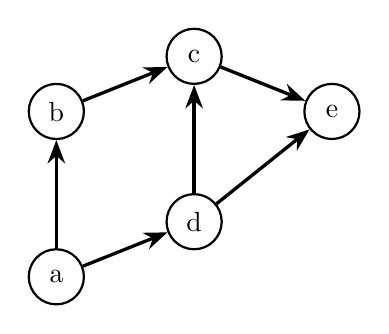
\begin{tikzpicture}[scale=0.7]
            \begin{scope}[every node/.style={circle,thick,draw,minimum size=\nodesize}]
                \node (a) at (0,0) {a};
                \node (b) at (0,3) {b};
                \node (c) at (2.5,4) {c};
                \node (d) at (2.5,1) {d};
                \node (e) at (5,3) {e};
            \end{scope}

            \begin{scope}[>={Stealth[black]},,
                every edge/.style={draw=black,very thick}]
                \path [->] (a) edge node {} (b);
                \path [->] (b) edge node {} (c);
                \path [->] (a) edge node {} (d);
                \path [->] (d) edge node {} (c);
                \path [->] (d) edge node {} (e);
                \path [->] (c) edge node {} (e);
            \end{scope}
            \end{tikzpicture}
    \end{figure}

    \bigskip

    \begin{block}{Definizione}
        Se $\langle a,b \rangle \in E \implies b$ è un nodo \emph{figlio} di $a$.
    \end{block}
\end{frame}

\begin{frame}\frametitle{Bisimulazione}
    \bisimulation

    \bigskip

    \begin{figure}
        \begin{subfigure}{0.55\textwidth}
            \centering
            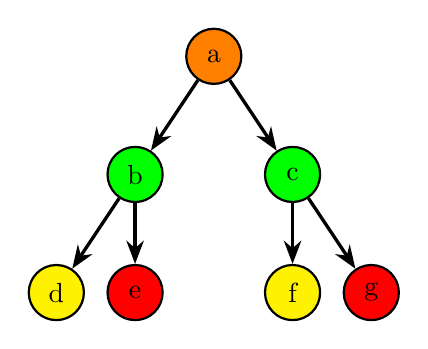
\begin{tikzpicture}[scale=0.5]
                \begin{scope}[every node/.style={circle,thick,draw,minimum size=\nodesize}]
                    \node[fill=orange] (a) at (0,6) {a};
                    \node[fill=green] (c) at (2,3) {c};
                    \node[fill=green] (b) at (-2,3) {b};
                    \node[fill=yellow] (d) at (-4,0) {d};
                    \node[fill=red] (e) at (-2,0) {e};
                    \node[fill=yellow] (f) at (2,0) {f};
                    \node[fill=red] (g) at (4,0) {g};
                \end{scope}

                \begin{scope}[>={Stealth[black]},
                    every edge/.style={draw=black,very thick}]
                    \path [->] (a) edge node {} (b);
                    \path [->] (a) edge node {} (c);

                    \path [->] (b) edge node {} (d);
                    \path [->] (b) edge node {} (e);

                    \path [->] (c) edge node {} (f);
                    \path [->] (c) edge node {} (g);
                \end{scope}
            \end{tikzpicture}
        \end{subfigure}
        \hfill
        \begin{subfigure}{0.44\textwidth}
            \begin{align*}
                \mathcal{B} = &\{(a,a), (b,c), (e,g), (d,f)\}
            \end{align*}
        \end{subfigure}
    \end{figure}
\end{frame}

\begin{frame}\frametitle{Massima bisimulazione}
    \begin{block}{Definizione}
        La \emph{massima bisimulazione} su $G = (V,E)$ è la relazione $\mathcal{B}_\mathcal{M}$ tale che:
        \begin{gather*}
            \mathcal{R} \subseteq \mathcal{B}_\mathcal{M} \quad \text{ per ogni bisimulazione } \mathcal{R} \text{ su } G.
        \end{gather*}
    \end{block}

    \bigskip\bigskip

    Si può dimostrare che:
    \begin{itemize}
        \item $\displaystyle \mathcal{B}_\mathcal{M} \,\,\,\,\,= \bigcup_{\substack{\mathcal{R} \text{ è una}\\\text{bisimulazione}}} \mathcal{R}$;
        \item $\mathcal{B}_\mathcal{M}$ è ancora una \emph{bisimulazione};
        \item La \emph{massima bisimulazione} è \textbf{unica};
        \item $\mathcal{B}_\mathcal{M}$ è una \emph{relazione di equivalenza}

        $\implies$ induce un partizionamento su $V$.
    \end{itemize}
\end{frame}

\begin{frame}\frametitle{Algoritmi per il calcolo della massima bisimulazione}
    \textbf{Non incrementali}
    \begin{itemize}
        \item Algoritmo di Paige-Tarjan;
        \item Algoritmo di Dovier-Piazza-Policriti;

        \qquad $\mathcal{B}_\mathcal{M}(u,v) \implies$ \texttt{rank}$(u) =$ \texttt{rank}$(v)$.
    \end{itemize}

    \bigskip

    \textbf{Incrementali}
    \begin{itemize}
        \item Algoritmo incrementale di Saha.
    \end{itemize}
\end{frame}

\begin{frame}[fragile]\frametitle{BisPy}
    \begin{itemize}
        \item Python 3
        \item Open source (\url{https://github.com/fAndreuzzi/BisPy})
    \end{itemize}


    \begin{example}
        \begin{verbatim}
        from bispy import paige_tarjan

        # creazione del grafo
        graph = networkx.balanced_tree(2,3)

        # calcolo della massima bisimulazione
        paige_tarjan(graph)

        >>> [(7, 8, 9, 10, 11, 12, 13, 14), (3, 4, 5, 6),
            (1, 2), (0,)]
        \end{verbatim}
    \end{example}
\end{frame}

\begin{frame}\frametitle{Risultati sperimentali I}
    \begin{figure}[b!]
        \centering
        \captionsetup[subfigure]{labelformat=empty}
        \begin{subfigure}{0.49\textwidth}
            \begin{tikzpicture}
                \begin{axis}[
                    axis on top,
                    width=\textwidth,
                    ytick style={draw=none},
                    xtick style={draw=none},
                    legend cell align={left},
                    legend style={fill=white,opacity=0.8, at={(0,0.69)},anchor=south west, legend columns=1},
                    xmode=log,
                    ymode=log,
                    ylabel={Secondi},
                    xlabel={Numero di nodi},
                    grid=major,
                    title={Alberi bilanciati}
                ]
                \addplot table[x=x,y=y] {../experiments/time/tree/pta.txt};
                \addlegendentry{PT}
                \addplot table[x=x,y=y] {../experiments/time/tree/fba.txt};
                \addlegendentry{DPP}
                \end{axis}
            \end{tikzpicture}
        \end{subfigure}
        \hfill
        \begin{subfigure}{0.49\textwidth}
            \centering
            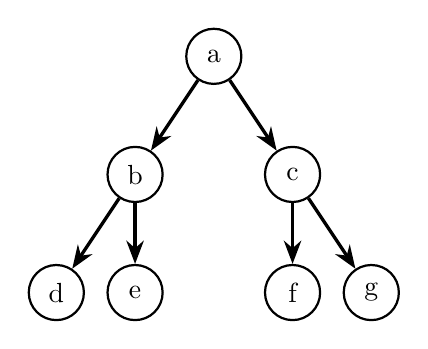
\begin{tikzpicture}[scale=0.5]
                \begin{scope}[every node/.style={circle,thick,draw,minimum size=\nodesize}]
                    \node (a) at (0,6) {a};
                    \node (c) at (2,3) {c};
                    \node (b) at (-2,3) {b};
                    \node (d) at (-4,0) {d};
                    \node (e) at (-2,0) {e};
                    \node (f) at (2,0) {f};
                    \node (g) at (4,0) {g};
                \end{scope}

                \begin{scope}[>={Stealth[black]},
                    every edge/.style={draw=black,very thick}]
                    \path [->] (a) edge node {} (b);
                    \path [->] (a) edge node {} (c);

                    \path [->] (b) edge node {} (d);
                    \path [->] (b) edge node {} (e);

                    \path [->] (c) edge node {} (f);
                    \path [->] (c) edge node {} (g);
                \end{scope}
            \end{tikzpicture}
            \caption{Un albero bilanciato.}
        \end{subfigure}
    \end{figure}
\end{frame}

\begin{frame}\frametitle{Risultati sperimentali II}
    \begin{figure}
        \centering
        \begin{subfigure}{0.48\textwidth}
            \begin{tikzpicture}
                \begin{axis}[
                    axis on top,
                    width=\textwidth,
                    legend style={nodes={scale=0.7, transform shape}, fill=white,opacity=0.8, at={(0,0.68)},anchor=south west, legend columns=1},
                    legend cell align={left},
                    ytick style={draw=none},
                    xtick style={draw=none},
                    xlabel={Numero di nodi},
                    ylabel={Secondi},
                    ymode=log,
                    grid=major,
                    title={Tempo medio punto 4.}
                ]
                \addplot table[x=x,y=y] {../experiments/time/saha/random/mean_0_0.txt};
                \addlegendentry{Paige-Tarjan}
                \addplot table[x=x,y=y] {../experiments/time/saha/random/mean_0_1.txt};
                \addlegendentry{DPP}
                \addplot table[x=x,y=y] {../experiments/time/saha/random/mean_0_2.txt};
                \addlegendentry{Saha}
            \end{axis}
            \end{tikzpicture}
        \end{subfigure}
        \hfill
        \begin{subfigure}{0.48\textwidth}
            \underline{\Large 100 volte}:
            \begin{enumerate}
                \item Generazione grafo \emph{randomico};
                \item Calcolo massima bisimulazione (per l'algoritmo di Saha);
                \item Aggiunta arco \emph{randomico};
                \item \textbf{Aggiornamento} massima bisimulazione (con \emph{PT}, \emph{DPP}, \emph{Saha}).
            \end{enumerate}
        \end{subfigure}
    \end{figure}
\end{frame}

\begin{frame}\frametitle{Risultati sperimentali III}
    \begin{figure}
        \centering
        \begin{tikzpicture}
            \begin{axis}[
                ybar stacked,
                axis on top,
                bar width=3pt,
                width=\textwidth,
                legend cell align={left},
                height=7cm,
                ytick style={draw=none},
                xtick style={draw=none},
                enlargelimits=0.01,
                xlabel={Indice esperimento},
                xlabel style={font=\large},
                ylabel={Secondi},
                xticklabels={,,},
                title={100 grafi randomici (2000 nodi)}
            ]
            \addplot table[x=x,y=y] {../experiments/time/saha/random/scatter_1_0.txt};
            \addlegendentry{Paige-Tarjan}
            \addplot table[x=x,y=y] {../experiments/time/saha/random/scatter_1_2.txt};
            \addlegendentry{Saha}
        \end{axis}
        \end{tikzpicture}
    \end{figure}
\end{frame}

\begin{frame}\frametitle{Risultati sperimentali IV}
    \centering
    \begin{figure}
        \begin{tikzpicture}
            \begin{axis}[
                ybar stacked,
                axis on top,
                width=\textwidth,
                legend cell align={left},
                height=7cm,
                bar width=3pt,
                xticklabels={,,},
                ytick style={draw=none},
                xtick style={draw=none},
                xlabel style={font=\large},
                ylabel={Secondi},
                ylabel style={font=\large},
                enlargelimits=0.01,
                xlabel={Indice esperimento},
                title={Aggiunta di un arco randomico ad alberi bilanciati}
            ]
            \addplot table[x=x,y=y] {../experiments/time/saha/tree/scatter_0.txt};
            \addlegendentry{Paige-Tarjan}
            \addplot table[x=x,y=y] {../experiments/time/saha/tree/scatter_1.txt};
            \addlegendentry{Dovier-Piazza-Policriti}
            \addplot table[x=x,y=y] {../experiments/time/saha/tree/scatter_2.txt};
            \addlegendentry{Saha}
            \begin{scope}[on background layer]
                \fill[green,opacity=0.1] ({rel axis cs:0,0}) rectangle ({rel axis cs:0.04,1});
                \fill[cyan,opacity=0.1] ({rel axis cs:0.04,0}) rectangle ({rel axis cs:0.09,1});
                \fill[lightgray,opacity=0.1] ({rel axis cs:0.09,0}) rectangle ({rel axis cs:0.14,1});
                \fill[magenta,opacity=0.1] ({rel axis cs:0.14,0}) rectangle ({rel axis cs:0.26,1});
                \fill[lime,opacity=0.1] ({rel axis cs:0.26,0}) rectangle ({rel axis cs:0.68,1});
                \fill[orange,opacity=0.1] ({rel axis cs:0.68,0}) rectangle ({rel axis cs:0.81,1});
                \fill[pink,opacity=0.1] ({rel axis cs:0.81,0}) rectangle ({rel axis cs:0.89,1});
                \fill[teal,opacity=0.1] ({rel axis cs:0.89,0}) rectangle ({rel axis cs:0.92,1});
                \fill[teal,opacity=0.1] ({rel axis cs:0.92,0}) rectangle ({rel axis cs:1,1});
            \end{scope}
            \end{axis}
        \end{tikzpicture}
    \end{figure}
\end{frame}

\begin{frame}\frametitle{Conclusione}
    Il software sviluppato ha consentito di osservare ed analizzare il comportamento degli algoritmi per varie tipologie di grafi.

    \bigskip\bigskip

    \textbf{Sviluppi futuri}
    \begin{itemize}
        \item Ricalcolo incrementale della massima bisimulazione dopo la \textbf{rimozione} di un arco;
        \item \emph{Labeled edges};
        \item Migliore integrazione con altre librerie (\texttt{NetworkX});
        \item Utilizzare \texttt{Cython} per parti critiche del codice.
    \end{itemize}
\end{frame}

\end{document}
